% \documentclass[twocolumn]{article}
\documentclass[]{article}
\usepackage[left=20mm, right=20mm, top=20mm, bottom=20mm]{geometry}
\usepackage{lipsum}  % This package generates filler text.
\usepackage{amsmath} % For mathematical formulas.
\usepackage{graphicx} % For including figures.
\usepackage{authblk} % For author and affiliation blocks.
\usepackage[english]{babel}
\usepackage{graphicx} % Required for inserting images
\usepackage{subcaption}
\usepackage{algorithm}
\usepackage{algorithmicx}
\usepackage{algpseudocode}
\usepackage[T1]{fontenc}
\usepackage[utf8]{inputenc}
\usepackage{url}
\usepackage{hyperref}
\usepackage{parskip}
\usepackage{xcolor}
\usepackage{amssymb}
\usepackage{comment}
\usepackage{multicol}
\usepackage{svg}
\usepackage{flushend}


\usepackage[
backend=biber,
style=alphabetic,
sorting=ydnt
]{biblatex} %Imports biblatex package
\addbibresource{reports/references.bib} %Import the bibliography file
\setlength\bibitemsep{0.5\baselineskip}

\hypersetup{
    colorlinks=true,
    urlcolor=blue,
    linkcolor=black
}

\newcommand{\C}{\mathbb{C}}
\newcommand{\R}{\mathbb{R}}
\newcommand{\Q}{\mathbb{Q}}
\newcommand{\Z}{\mathbb{Z}}
\newcommand{\N}{\mathbb{N}}
\newcommand{\proofend}{\hfill $\square$}
\newcommand{\deltach}{\hat{\delta}}

\title{\textbf{IFT 3710 - Team "GANg"} \\ 
\textbf{Data Augmentation for Cell Segmentation}}

\author[1]{Bio Samir Gbian}
\author[1]{Kamen Damov}
\author[1]{Simon Langlois}
\author[1]{Guillaume Genois}
\author[1]{Johann Sourou}
\affil{Departement of Computer Science and Operations Research}
\affil[1]{University of Montreal}

\begin{document}
\maketitle

\href{https://github.com/KamenDamov/IFT3710-Advanced-Project-in-ML-AI}{GitHub Code Repository}

\section{Preprocessing}
This section details the image transformation pipeline used in a microscopy image segmentation framework based on the MONAI (Medical Open Network for AI) library. The transformations are applied to both the input images and their corresponding segmentation labels to augment the dataset and improve model generalization.\\
\textbf{Training Transformations}
The training pipeline incorporates both spatial and intensity transformations to create a diverse set of training samples:
\begin{align}
    \mathcal{T}_{train} = {T_1, T_2, \ldots, T_n}
\end{align}
where each $T_i$ represents a specific transformation operation.\\
\textbf{Loading and Channel Transformations}
\begin{align}
T_1 &= \textbf{LoadImaged}(\text{keys}=[\text{"img", "label"}]) \\
T_2 &= \textbf{AddChanneld}(\text{keys}=[\text{"label"}]) \\
T_3 &= \textbf{AsChannelFirstd}(\text{keys}=[\text{"img"}]
\end{align}
These initial transformations handle the loading of images and labels, ensuring the proper channel arrangements. The images are originally in format $(H, W, 3)$ and are transformed to $(3, H, W)$, while labels are expanded from $(H, W)$ to $(1, H, W)$.\\
\textbf{Intensity Normalization}
\begin{align}
    T_4 = \textbf{ScaleIntensityd}(\text{keys}=[\text{"img"}])
\end{align}
This transformation normalizes the intensity values of the input images, scaling them to a standardized range.\\
\textbf{Spatial Transformations}
\begin{align}
    T_5 &= \textbf{SpatialPadd}(\text{keys}=[\text{"img", "label"}]),\\ %\text{spatial_size}=256) \
    T_6 &= \textbf{RandSpatialCropd}(\text{keys}=[\text{"img", "label"}]),\\ %\text{roi_size}=256) \
    T_7 &= \textbf{RandAxisFlipd}(\text{keys}=[\text{"img", "label"}]),\\ %\text{prob}=0.5) \
    T_8 &= \textbf{RandRotate90d}(\text{keys}=[\text{"img", "label"}]), %\text{prob}=0.5, \text{spatial_axes}=[0, 1])
\end{align}
These transformations modify the spatial properties of the images and labels through padding, cropping, flipping, and rotation operations, which introduces geometric variability into the training set.\\
\textbf{Intensity Augmentations}
\begin{align}
    T_9 &= \textbf{RandGaussianNoised}(\text{keys}=[\text{"img"}]),\\ %\text{prob}=0.25, \text{mean}=0, \text{std}=0.1) \
    T_{10} &= \textbf{RandAdjustContrastd}(\text{keys}=[\text{"img"}]),\\ %\text{prob}=0.25, \text{gamma}=(1, 2)) \
    T_{11} &= \textbf{RandGaussianSmoothd}(\text{keys}=[\text{"img"}]),\\ %\text{prob}=0.25, \text{sigma_x}=(1, 2)) \
    T_{12} &= \textbf{RandHistogramShiftd}(\text{keys}=[\text{"img"}]), %\text{prob}=0.25, \text{num_control_points}=3)
\end{align}
These transformations modify the intensity characteristics of the images through noise addition, contrast adjustment, smoothing, and histogram manipulation, simulating various imaging conditions.\\
\textbf{Advanced Spatial Transformations}
\begin{align}
T_{13} = \textbf{RandZoomd}(&\text{keys}=[\text{"img", "label"}]), %\text{prob}=0.15, 
%&\text{min_zoom}=0.8, \text{max_zoom}=1.5, \text{mode}=[\text{"area", "nearest"}])
\end{align}
This transformation randomly scales the images and labels, creating variations in object size and resolution.\\
\textbf{Type Conversion}
\begin{align}
T_{14} = \textbf{EnsureTyped}(\text{keys}=[\text{"img", "label"}])
\end{align}
This final transformation ensures that the data types are compatible with the PyTorch framework.\\
\textbf{Validation Transformations}
The validation pipeline is simpler and focuses on preparing the data without augmentation:
\begin{align}
\mathcal{T}_{val} = {T'_1, T'_2, \ldots, T'_m}
\end{align}
where each $T'_j$ represents a validation-specific transformation operation.
\begin{align}
    T'_1 &= \textbf{LoadImaged}(\text{keys}=[\text{"img", "label"}]) \\
    T'_2 &= \textbf{AddChanneld}(\text{keys}=[\text{"label"}]) \\
    T'_3 &= \textbf{AsChannelFirstd}(\text{keys}=[\text{"img"}]),\\ %\text{channel_dim}=-1) \
    T'_4 &= \textbf{ScaleIntensityd}(\text{keys}=[\text{"img"}]), \\
    T'_5 &= \textbf{EnsureTyped}(\text{keys}=[\text{"img", "label"}])
\end{align}
The validation transformations maintain the same preprocessing steps but exclude the augmentation operations to ensure consistent evaluation.\\

\section{Models}

\subsection{U-Net}

\subsection{Cellpose 3.0}


\section{Data Augmentation}

A challenge that was flagged by the other competitors was the inefficiency of using unlabeled data. We try a novel way to generate pseudo masks. We explore two ways to do so.
\subsection{Pix2Pix}
Generative Adversarial Networks (GANs) have been widely used for image-to-image translation tasks, and conditional GANs (cGANs) extend this concept by learning a mapping from a source domain \( X \) to a target domain \( Y \) given paired data. In this work, we leverage the Pix2Pix architecture, a cGAN designed for paired image translation, to generate pseudo-masks from raw images.

Instead of employing a traditional segmentation model, we fine-tune Pix2Pix using a corpus of labeled data consisting of \textit{(raw image, segmentation mask)} pairs. The generator \( G \) in the Pix2Pix framework learns to map an input raw image \( x \in X \) to a synthetic segmentation mask \( \hat{y} \in Y \), while the discriminator \( D \) evaluates the realism of the generated mask by distinguishing it from real ground truth segmentation masks. This adversarial setup optimizes the generator to produce segmentation masks that closely resemble human-labeled annotations.

The objective function for Pix2Pix is formulated as:
\begin{equation}
    \mathcal{L}_{\text{cGAN}}(G, D) = \mathbb{E}_{(x,y) \sim p_{\text{data}}(x,y)} \left[ \log D(x, y) \right] + \mathbb{E}_{x \sim p_{\text{data}}(x)} \left[ \log (1 - D(x, G(x))) \right],
\end{equation}
where \( G \) attempts to minimize this loss while \( D \) aims to maximize it.

To ensure that the generated segmentation masks remain faithful to the structural information in the input image, we incorporate an additional \( L_1 \) loss:
\begin{equation}
    \mathcal{L}_{L_1}(G) = \mathbb{E}_{(x,y) \sim p_{\text{data}}(x,y)} \left[ \| y - G(x) \|_1 \right].
\end{equation}
Thus, the full objective function is:
\begin{equation}
    G^* = \arg \min_G \max_D \mathcal{L}_{\text{cGAN}}(G, D) + \lambda \mathcal{L}_{L_1}(G),
\end{equation}
where \( \lambda \) is a weighting factor controlling the influence of the \( L_1 \) loss.

Once the Pix2Pix model is trained, we apply the generator to previously unlabeled raw images to produce synthetic segmentation masks, which we refer to as \textit{pseudo-masks}. These pseudo-masks will then be integrated into a larger training set to improve the performance of a dedicated segmentation model. This approach allows us to expand the labeled dataset without requiring additional manual annotations, leveraging adversarial learning to refine mask generation. That said, we have issues stabilizing the training of this model, a recurring issue with GANs. 

\subsection{SAM-2}



\subsection{Image captionning}



\section{Résultat preliminaire}
Voici un exemple de résultat obtenu après avoir effectué le preprocessing:

\begin{figure}[!h]
    \begin{subfigure}[b]{0.45\textwidth}
        \centering
        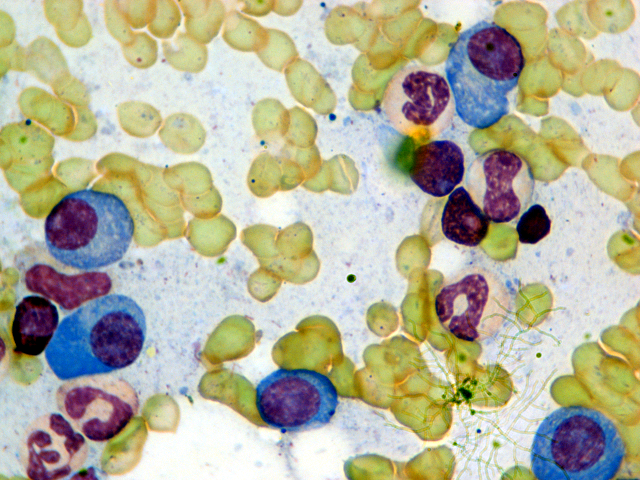
\includegraphics[scale=0.5]{reports/images/cell_00001.png}
        \caption{Original image, 640 x 480}
    \end{subfigure}
    \hfill
    \begin{subfigure}[b]{0.45\textwidth}
        \centering
        \includegraphics[scale=0.5]{reports/images/transformed_images_cell_00001.png}
        \caption{Transformed image, 216 x 216}
    \end{subfigure}
    \label{fig:transformed_images}
\end{figure}

\section{Conclusion}
The comprehensive transformation pipeline described in this report facilitates robust training of deep learning models for microscopy image segmentation. The training transformations introduce diverse variations to the input data, enhancing the model's ability to generalize to unseen images, while the validation transformations ensure fair and consistent evaluation. This approach aligns with best practices in medical image analysis, where data augmentation is crucial due to the limited availability of annotated data.

\end{document}